\chapter{Benchmark results}
\label{cha:results}

This chapter reports benchmark performance for the forecasting methods considered in the thesis. The evaluation follows the protocol defined in Chapter~\ref{cha:protocol} and includes both aggregate scores and examples of forecast trajectories.

\section{Numerical results}

This section compares skill score and ramp NMAE across reference forecasts, numerical models, time-series foundation models, and multimodal forecasters.

\subsection{Reference forecasts}

Table~\ref{tab:results-reference} reports three rule-based reference forecasts under the common UK protocol. They show how much skill follows from carrying forward recent power or exploiting its recurring daily pattern.

\begin{table}[htbp]\centering
\begin{tabular}{lcc}\hline
Method & Skill (\%) & Ramp NMAE \\\hline
Persistence & 1.41 & 0.2550 \\
Seasonal naive & 10.68 & 0.2056 \\
Hourly climatology & 23.37 & 0.1665 \\\hline
\end{tabular}
\caption{Rule-based reference forecasts on the primary cross-plant test set. Higher skill and lower ramp NMAE are better.}\label{tab:results-reference}
\end{table}

The scores rise from persistence through seasonal naive to hourly climatology, showing the value of recurring daily structure. Hourly climatology also lowers ramp error. Its fixed per-hour mean cannot adapt to local conditions that change from one forecast day to the next.

\subsection{Tabular models}

The models in Table~\ref{tab:results-tabular} use engineered lagged numerical features. They test how far learned tabular representations can improve on the rule-based references without modeling the input as a sequence.

\begin{table}[htbp]\centering
\begin{tabular}{lcc}\hline
Method & Skill (\%) & Ramp NMAE \\\hline
LightGBM & 38.54 & 0.1672 \\
TabPFN & 40.63 & 0.1631 \\\hline
\end{tabular}
\caption{Tabular models on the primary cross-plant test set. Higher skill and lower ramp NMAE are better.}\label{tab:results-tabular}
\end{table}

\subsection{Supervised sequence models}

Table~\ref{tab:results-supervised} lists numerical sequence models trained on the benchmark training plants.

\begin{table}[htbp]\centering
\begin{tabular}{lcc}\hline
Method & Skill (\%) & Ramp NMAE \\\hline
iTransformer & 52.57 & 0.1445 \\
PatchTST & 45.81 & 0.1543 \\
TFT & 42.64 & 0.1605 \\
MLP baseline & 42.19 & 0.1624 \\
DLinear & 32.31 & 0.1746 \\\hline
\end{tabular}
\caption{Supervised numerical sequence baselines. TFT denotes Temporal Fusion Transformer.}\label{tab:results-supervised}
\end{table}

\subsection{Time-series foundation models zero-shot}

Table~\ref{tab:results-foundation-transfer} lists time-series foundation models evaluated without task-specific fitting.

\begin{table}[htbp]\centering
\begin{tabular}{lcc}\hline
Method & Skill (\%) & Ramp NMAE \\\hline
Chronos-2 zero-shot & 47.37 & 0.1544 \\
TiRex zero-shot & 28.73 & 0.1826 \\
TimesFM zero-shot & 27.08 & 0.1902 \\
TTM zero-shot & -8.07 & 0.2922 \\\hline
\end{tabular}
\caption{Protocol-aligned zero-shot time-series foundation models.}\label{tab:results-foundation-transfer}
\end{table}

Chronos-2 has the strongest zero-shot result in this table, with skill 47.37 and ramp NMAE 0.1544. TTM's negative zero-shot skill shows that pretraining alone does not guarantee transfer to this plant-disjoint task.

\subsection{Adapted time-series foundation models}

Table~\ref{tab:results-foundation-adaptation} compares models that adapt a pretrained time-series foundation model to the training plants, either by fine-tuning or with a covariate adapter.

\begin{table}[htbp]\centering
\begin{tabular}{lcc}\hline
Method & Skill (\%) & Ramp NMAE \\\hline
Chronos-2 fine-tuned & 52.30 & 0.1506 \\
CoRA & 37.98 & 0.1624 \\
TTM fine-tuned & 36.01 & 0.1716 \\\hline
\end{tabular}
\caption{Protocol-aligned time-series foundation-model adaptation results.}\label{tab:results-foundation-adaptation}
\end{table}

The fine-tuned Chronos-2 control has skill 52.30 and ramp NMAE 0.1506. Its score is 4.93 points above the zero-shot Chronos-2 result, and its ramp NMAE is lower by 0.0038. By comparison, iTransformer has similar skill but lower ramp NMAE.

\subsection{Retrieval methods}

Table~\ref{tab:retrieval-native} reports results for TS-RAG~\cite{tsrag} and Cross-RAG~\cite{crossrag}. Both methods retrieve related historical power sequences from an external store to condition the forecast on past similar production regimes.

\begin{table}[htbp]\centering
\begin{tabular}{lcc}\hline
Method & Skill (\%) & Ramp NMAE \\\hline
TS-RAG & 47.79 & 0.1568 \\
Cross-RAG & 47.68 & 0.1545 \\\hline
\end{tabular}
\caption{Retrieval-augmented forecasting models on the cross-plant test set.}\label{tab:retrieval-native}
\end{table}

Both retrieval methods achieve skill scores near 47.7\%, placing them slightly above zero-shot Chronos-2 (47.37\%) and above supervised sequence baselines such as PatchTST (45.81\%) and TFT (42.64\%). TS-RAG reaches slightly higher overall skill at 47.79\%, while Cross-RAG obtains a lower ramp NMAE of 0.1545, matching the ramp error of zero-shot Chronos-2 (0.1544). Both methods score below fine-tuned Chronos-2 (52.30\%) and iTransformer (52.57\%), showing that retrieving similar historical trajectories provides useful reference context across plants without matching the accuracy of direct parameter adaptation.

\subsection{Multimodal baselines}

Table~\ref{tab:results-multimodal} reports benchmark results for MMTSFM and fine-tuned Aurora.

\begin{table}[htbp]\centering
\begin{tabular}{lcc}\hline
Method & Skill (\%) & Ramp NMAE \\\hline
Spatial-token & 55.10 & 0.1440 \\
Multi-anchor & 54.09 & 0.1463 \\
Pooled-image & 52.58 & 0.1487 \\
Aurora fine-tuned~\cite{aurora} & 40.52 & 0.1555 \\\hline
\end{tabular}
\caption{Multimodal benchmark results on the primary cross-plant test set. Higher skill and lower ramp NMAE are better.}\label{tab:results-multimodal}
\end{table}

The matched vision-off controls in Chapter~\ref{cha:ablations} test whether the fitted models depend on their visual pathways.

Spatial-token fusion has the highest skill score among the MMTSFM arms. Within the ladder, its ramp NMAE is 0.1440, compared with 0.1487 for pooled-image fusion and 0.1506 for the numerical control. Fine-tuned Aurora scores 40.52\% skill with 0.1555 ramp NMAE, providing a comparison from an atmospheric foundation model.

\subsection{Full payload feasibility result}

Full payload has one completed seed and a smaller eligible target set, with 163,559 scored target steps compared with 165,295 for the single-anchor arm. Because it requires cached imagery at all five daily anchors, origins missing a required entry are excluded. This smaller scored set can change the average error independently of the model. Its recorded score is therefore descriptive pending additional seeds and scoring both interfaces on their shared eligible windows.

\begin{table}[htbp]\centering
\begin{tabular}{lcc}\hline
Method & Skill (\%) & Ramp NMAE \\\hline
Full payload & 54.49 & 0.1458 \\\hline
\end{tabular}
\caption{Full payload feasibility result on its smaller eligible target set.}\label{tab:results-full-payload}
\end{table}

\subsection{Alternative multimodal baselines}

Table~\ref{tab:results-multimodal-context} reports results for five additional multimodal and vision-augmented forecasting models, spanning vision-language architectures, atmospheric foundation models, and convolutional networks.

\begin{table}[htbp]\centering
\begin{tabular}{lcc}\hline
Method & Skill (\%) & Ramp NMAE \\\hline
Time-VLM~\cite{timevlm} & 54.04 & 0.1374 \\
Solar-VLM~\cite{solarvlm} & 43.96 & 0.1514 \\
Aurora zero-shot~\cite{aurora} & 23.24 & 0.2051 \\
SUNSET~\cite{sunset} & 21.62 & 0.1757 \\
UniCast~\cite{unicast} & 12.11 & 0.2302 \\\hline
\end{tabular}
\caption{Alternative multimodal forecasting baselines on the cross-plant test set.}\label{tab:results-multimodal-context}
\end{table}

Time-VLM achieves 54.04\% skill, comparable to Multi-anchor (54.09\%) and Spatial-token fusion (55.10\%). It records the lowest ramp NMAE across all evaluated models at 0.1374, showing that rendering time series as visual plots allows the vision-language backbone to detect steep transitions and ramp events effectively. Solar-VLM attains 43.96\% skill and 0.1514 ramp NMAE, outperforming supervised models such as TFT (42.64\%) while trailing zero-shot Chronos-2 (47.37\%).

Atmospheric and convolutional models record lower overall skill. Zero-shot Aurora obtains 23.24\% skill and 0.2051 ramp NMAE. When fine-tuned on plant data, as shown in Table~\ref{tab:results-multimodal}, its skill rises to 40.52\% and ramp error drops to 0.1555, showing the importance of task adaptation for general weather representations. SUNSET achieves 21.62\% skill and 0.1757 ramp NMAE; its convolutional image pipeline improves upon simple persistence and climatology references, yet falls short of modern transformer architectures on held-out plants. UniCast scores 12.11\% skill and 0.2302 ramp NMAE, reflecting limited zero-shot transfer without installation-specific adaptation.

\section{Zero-shot transfer from the UK to the US fleet}

The preceding tables report the primary UK plant-disjoint benchmark. Table~\ref{tab:us-mmtsfm-transfer} reports the cross-region experiment: checkpoints trained on UK plants are evaluated on eight US plants with their parameters fixed. Plants 1283 and 51 are excluded by the dataset quality flags. All remaining US plants are unseen during model fitting. Power is resampled to 30-minute cadence, giving a twelve-step, six-hour horizon from fourteen days of local history. Each run scores the same 41,914 valid daylight targets. The four main arms use matched UK training seeds 42, 43, and 44, with plants weighted equally within each run and run scores then averaged across seeds.

% Recorded evaluations: baselines/results/mmtsfm_{s1,s2a,s2d,s2e}_goespvdaq_*_all_s{42,43,44}.json.
% Reference: baselines/results/smart_persistence_s2_goespvdaq_all.json.
% Interpretation and exact artifact links: report/BASELINE_TEST_REPORT.md, US transfer section.

\begin{table}[htbp]\centering
\small
\setlength{\tabcolsep}{6pt}
\begin{tabular}{@{}lccc@{}}\hline
Arm & Skill (\%) & NMAE & Ramp NMAE \\\hline
Numerical & 8.90 & 0.1719 & 0.1864 \\
Pooled-image & $-3.03$ & 0.1933 & 0.2008 \\
Spatial-token & 8.85 & 0.1745 & 0.1692 \\
Multi-anchor & 10.46 & 0.1657 & 0.1702 \\
Full payload & 3.46 & 0.1771 & 0.1786 \\\hline
\end{tabular}
\caption{Inference-only UK-to-US transfer on eight plants and 41,914 valid daylight targets. Main-arm entries are three-seed means. Full payload has seed 42 only. Skill uses the US Smart Persistence reference.}
\label{tab:us-mmtsfm-transfer}
\end{table}

Multi-anchor achieves the highest mean skill score at 10.46 percent and the lowest overall NMAE at 0.1657, improving on the numerical control at 8.90 percent skill and 0.1719 NMAE. It exceeds spatial-token fusion in skill across all three paired seeds. On ramp intervals, both structured visual architectures improve over the numerical baseline. Spatial-token fusion records the lowest ramp NMAE at 0.1692, followed closely by multi-anchor at 0.1702, compared with 0.1864 for the numerical control. The localized cloud information in spatial tokens and multi-temporal anchors helps the network anticipate steep power swings under unfamiliar US atmospheric conditions.

In contrast, pooled-image fusion yields negative skill at $-3.03$ percent and higher errors across the board, with an NMAE of 0.1933 and a ramp NMAE of 0.2008. Compressing the visual input into a single pooled token discards spatial gradients and makes the model sensitive to differences in sensor calibration between SEVIRI and GOES-16. By retaining spatial layout, spatial-token fusion matches the numerical control on overall skill ($8.85$ percent versus $8.90$ percent) while achieving lower ramp error. Multi-anchor fusion gains further by distributing tokens across five observation times, providing temporal progression across the context window.

The US full payload configuration uses 70 selected tokens at each of five daily anchors, fewer than the 98 tokens per anchor in the UK experiment. Its single-seed run attains 3.46 percent skill and 0.1786 ramp NMAE, tracking ramps better than the numerical baseline (0.1864) and pooled-image fusion (0.2008). Across the main arms, calibration reflects the regional transfer. Mean nominal 80 percent coverage ranges from 0.409 for spatial-token fusion to 0.523 for pooled-image fusion, while multi-anchor reaches 0.459, lower than the UK coverage levels. These eight plants provide evidence across different climatic zones, though they represent a quality-filtered subset observed over a single evaluation period.

\section{Visual inspection of the forecasts}

The result tables show overall performance, but they do not show where errors occur. Figure~\ref{fig:baseline-scatters} compares observed and predicted normalized power for fine-tuned Chronos-2, iTransformer, LightGBM, and fine-tuned Aurora. In each panel, observed power is on the horizontal axis and predicted power is on the vertical axis. Points on the dashed diagonal are accurate predictions. Points above it are overpredictions, and points below it are underpredictions. Colour shows where observations are most concentrated. The plots pool valid daylight observations from the 14 held-out plants. Benchmark scores weight plants equally, so the densest parts of a plot do not necessarily have the greatest influence on its score.

\begin{figure}[H]\centering
\begin{minipage}{0.48\textwidth}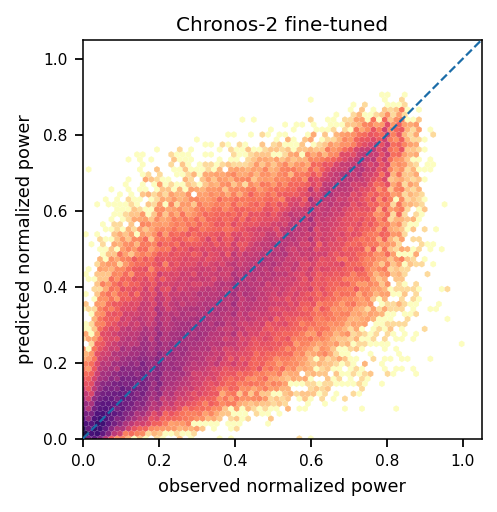
\includegraphics[width=\textwidth]{figures/scatter_mmtsfm_s1.png}\end{minipage}\hfill
\begin{minipage}{0.48\textwidth}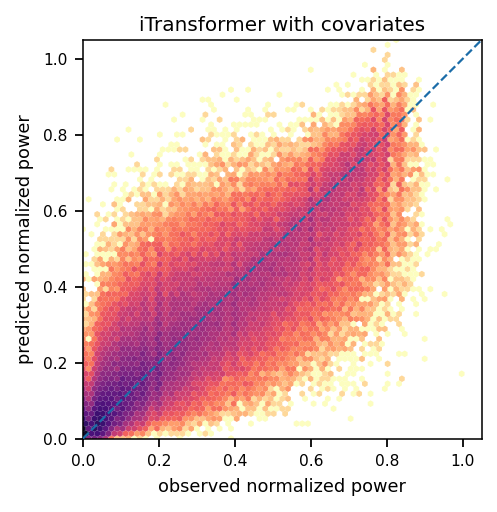
\includegraphics[width=\textwidth]{figures/scatter_itransformer.png}\end{minipage}\\[0.5em]
\begin{minipage}{0.48\textwidth}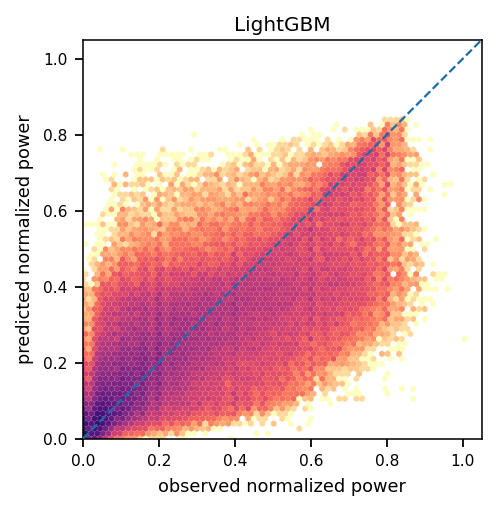
\includegraphics[width=\textwidth]{figures/scatter_lightgbm.png}\end{minipage}\hfill
\begin{minipage}{0.48\textwidth}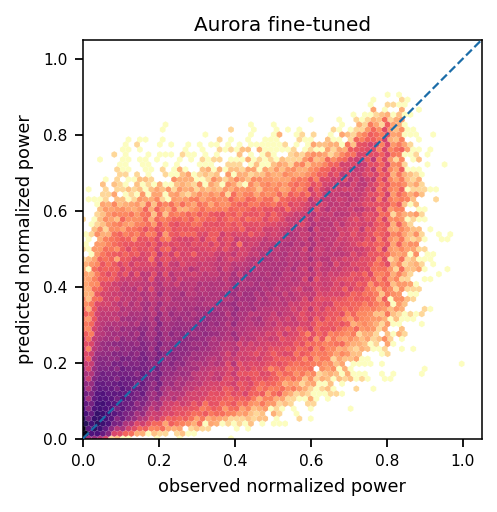
\includegraphics[width=\textwidth]{figures/scatter_aurora_ft.png}\end{minipage}
\caption{Predicted versus observed normalized power for four benchmark models. Colour shows observation density on a logarithmic scale. The dashed line marks perfect predictions.}
\label{fig:baseline-scatters}
\end{figure}

In all four panels, the densest observations follow the diagonal at low and moderate output. Predictions spread more widely as observed power rises. High observed values are often predicted too low. This is clearest for LightGBM, whose predictions level off before the observed range ends. iTransformer reaches higher predicted values, although its scatter remains broad. Fine-tuned Chronos-2 and Aurora also show underprediction near the upper end. Each panel contains positive predictions when observed output is close to zero. These patterns show where the models make errors that their aggregate scores cannot locate.

Figure~\ref{fig:mmtsfm-scatters} compares the three visual fusion arms on the same daylight observations and axes. It shows how the distribution of prediction errors changes across the fusion interfaces.

\begin{figure}[H]\centering
\begin{minipage}{0.32\textwidth}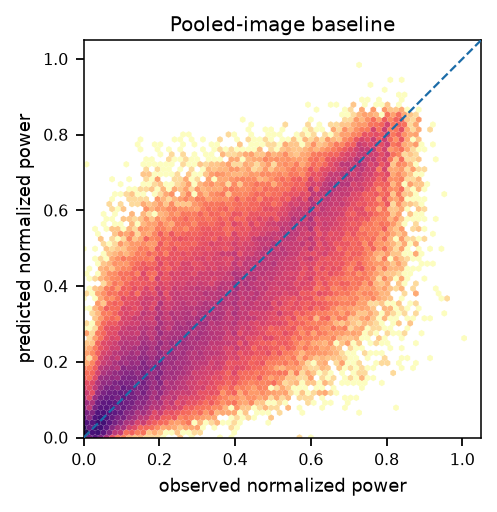
\includegraphics[width=\textwidth]{figures/scatter_mmtsfm_s2a.png}\end{minipage}\hfill
\begin{minipage}{0.32\textwidth}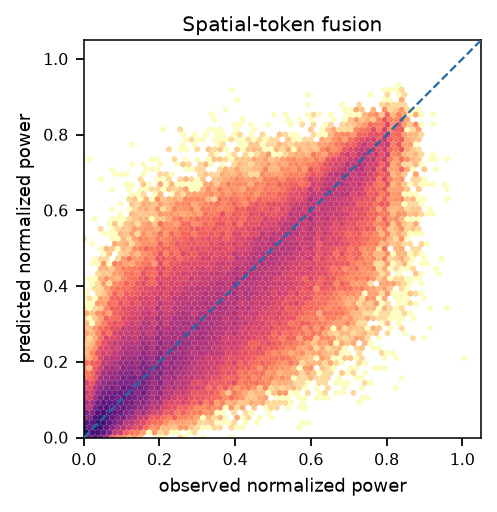
\includegraphics[width=\textwidth]{figures/scatter_mmtsfm_s2d.png}\end{minipage}\hfill
\begin{minipage}{0.32\textwidth}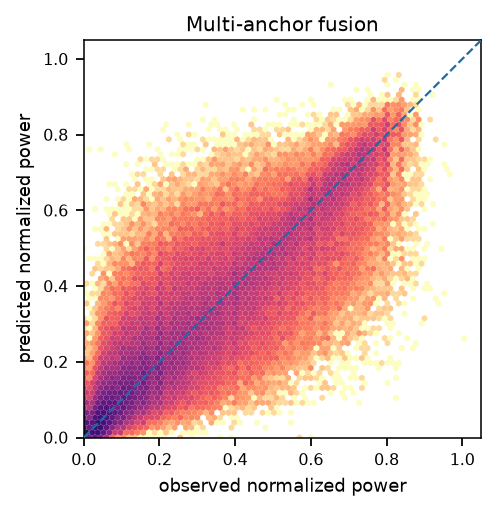
\includegraphics[width=\textwidth]{figures/scatter_mmtsfm_s2e.png}\end{minipage}
\caption{Predicted versus observed normalized power for the three visual fusion arms, shown with identical axes and daylight masking.}
\label{fig:mmtsfm-scatters}
\end{figure}

All three arms follow the overall rise in observed power. Their predictions spread apart at higher output. Pooled-image fusion has a broad cloud below the diagonal when observed power is high. Spatial-token fusion places more predictions near the diagonal in this range, although it still underpredicts some large values. The multi-anchor panel is more dispersed than the spatial-token panel and shows no comparable tightening around the diagonal. Each arm also makes some positive predictions when observed power is close to zero.

Figure~\ref{fig:tier-traces} follows three ramp windows from an evaluation plant. Each row shows the same window in both columns. The left column compares fine-tuned Chronos-2, iTransformer, LightGBM, and fine-tuned Aurora. The right compares pooled-image, spatial-token, and multi-anchor. The pale grey line at negative hours is observed power from the previous day. The break in the horizontal axis skips the intervening night. The dotted line at hour zero marks the forecast origin. To its right, the dark grey line is the observed outcome, and the coloured dashed lines are six-hour forecasts. Their direction, timing, and height show which changes each model follows or misses.

\begin{figure}[H]\centering
\begin{minipage}{0.48\textwidth}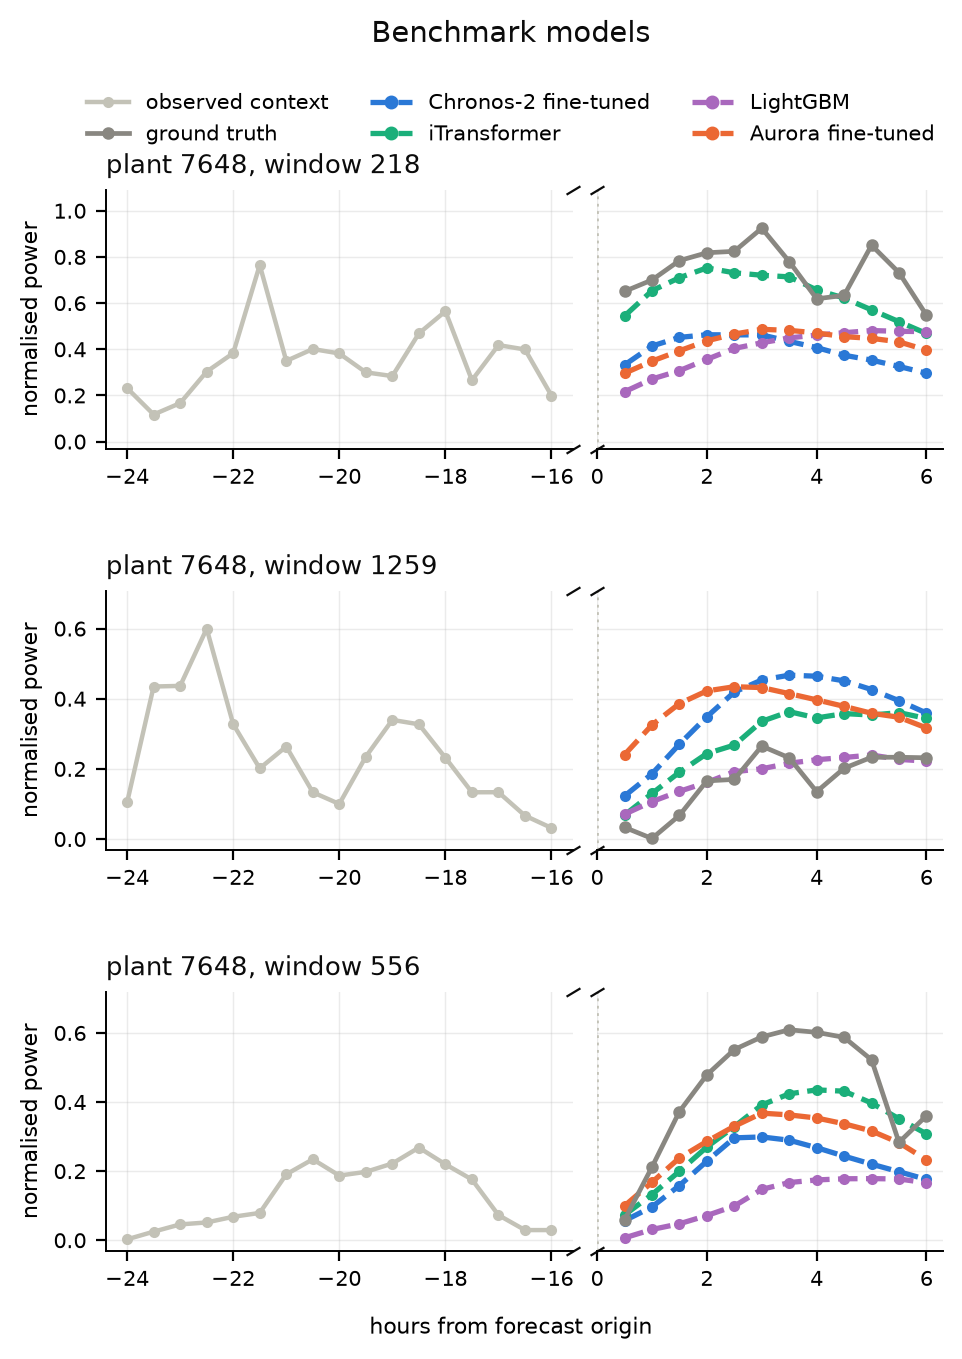
\includegraphics[width=\textwidth]{figures/traces_tsfm.png}\end{minipage}\hfill
\begin{minipage}{0.48\textwidth}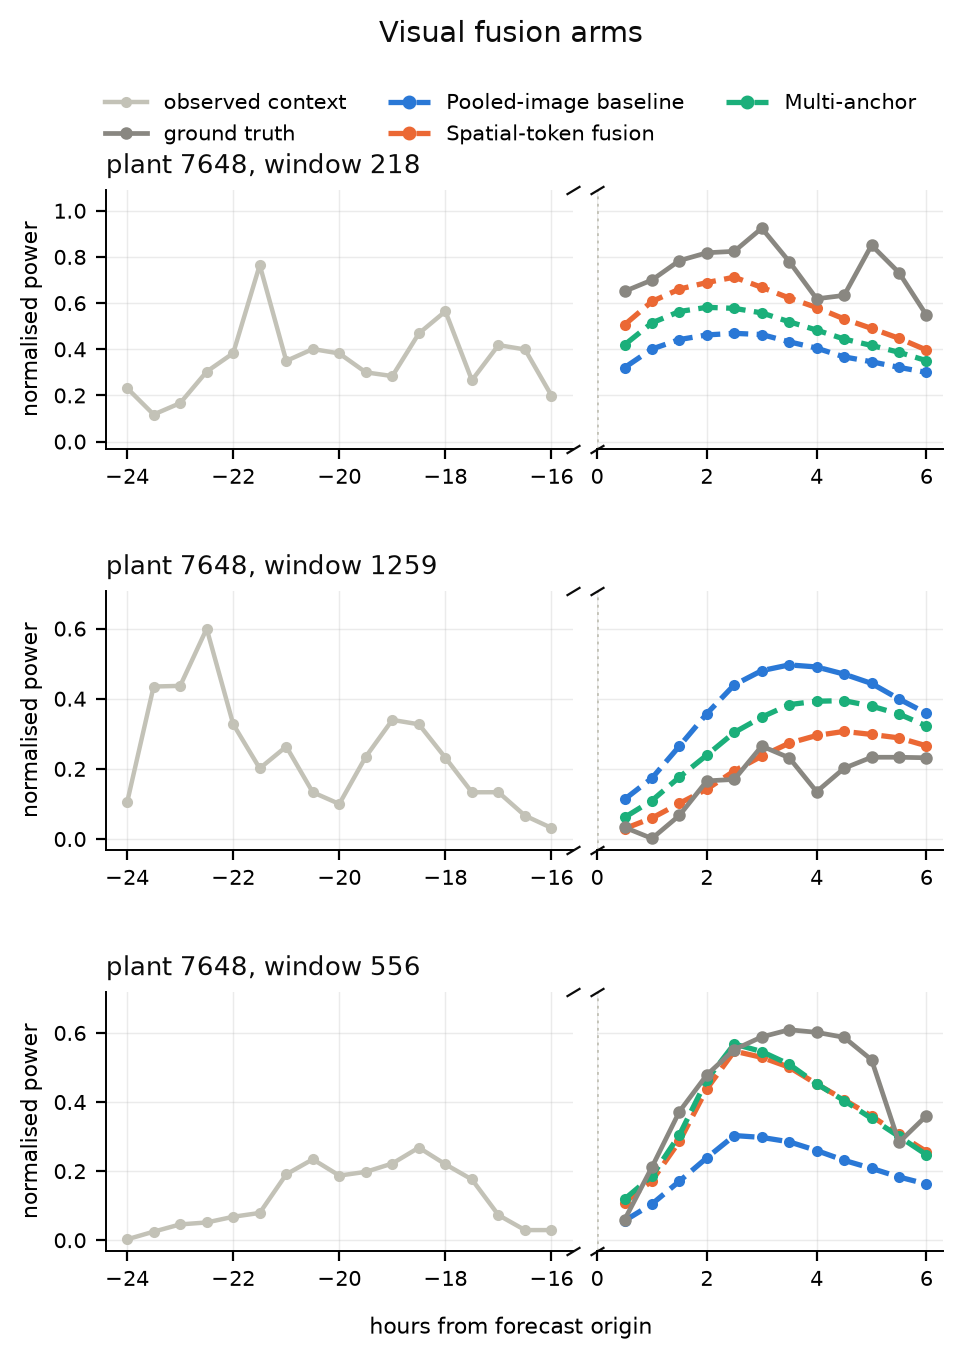
\includegraphics[width=\textwidth]{figures/traces_multimodal.png}\end{minipage}
\caption{Forecast trajectories for three ramp windows from plant 7648. The same windows appear in both columns.}
\label{fig:tier-traces}
\end{figure}

The three windows expose different errors. In window 218, the observed output rises above most forecasts. iTransformer comes closest to the peak among the benchmark models. Spatial-token fusion is closest among the visual arms. In window 1259, output remains low after a brief rise. LightGBM and spatial-token fusion follow that lower level more closely. Several other forecasts stay too high. In window 556, spatial-token and multi-anchor capture the sharp rise but still miss the peak. The pooled-image baseline and fine-tuned Chronos-2 produce flatter, lower forecasts for that window.

Figure~\ref{fig:worked-trace} shows a pronounced upward ramp within one six-hour forecast. It uses the same broken time axis as Figure~\ref{fig:tier-traces}. The pale grey segment shows observations from the previous day. The dark grey line on the right shows the outcome after the forecast origin. The coloured dashed lines show the model forecasts.

\begin{figure}[H]\centering
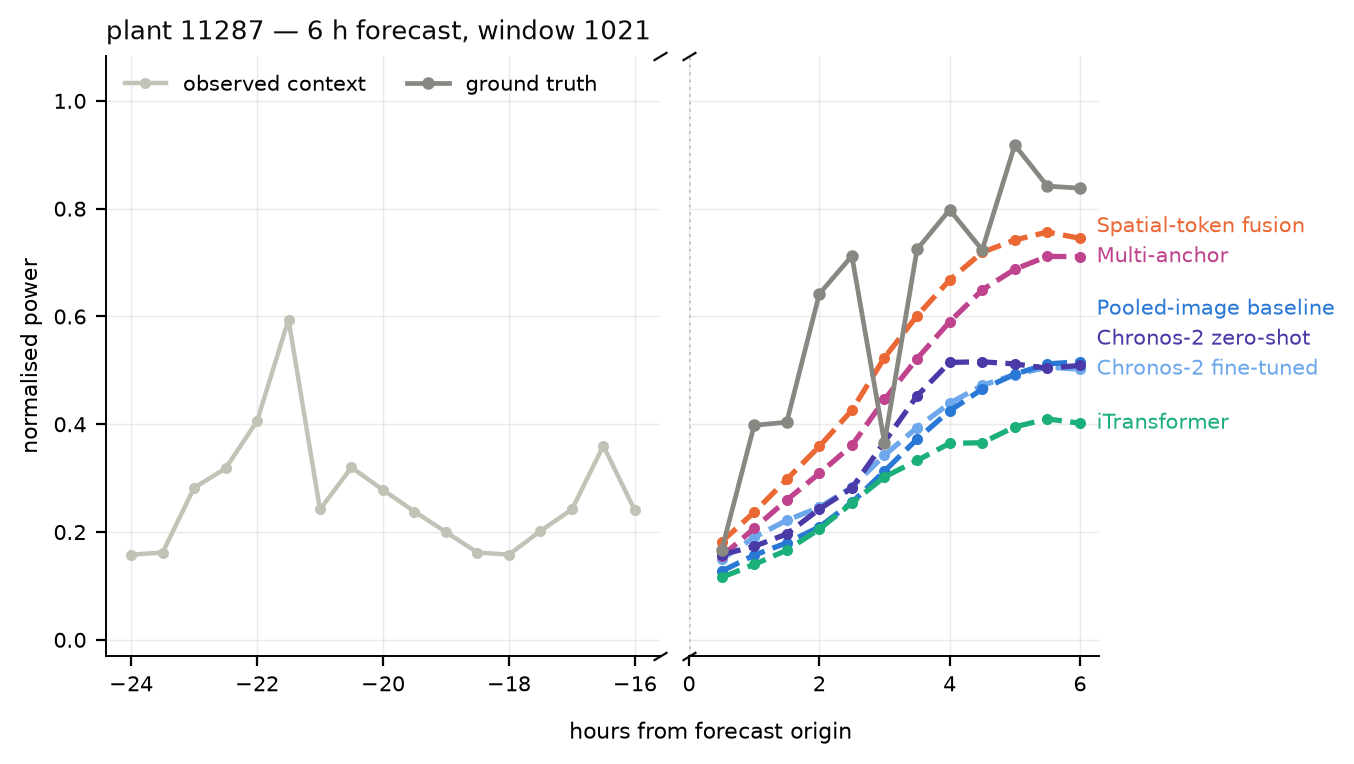
\includegraphics[width=0.94\textwidth]{figures/traces_comparison_11287_w1021.png}
\caption{Six-hour forecast across an upward ramp at plant 11287, window 1021.}
\label{fig:worked-trace}
\end{figure}

Observed power rises sharply after the forecast origin, with brief peaks around hours 2.5 and 5. Spatial-token fusion follows the overall climb but smooths those peaks; multi-anchor also rises, though at a lower level. The numerical control and pooled-image baseline flatten earlier. This trace shows how the forecasts differ during one ramp event.

The ramp comparisons above evaluate plants within the UK fleet where the models were trained. Figure~\ref{fig:us-traces} shifts focus to the cross-region transfer, displaying individual six-hour forecasts on unseen US plants. Each panel presents the daylight window with the greatest observed change between the first and last target step for the first three plants in the test partition. 

\begin{figure}[H]\centering
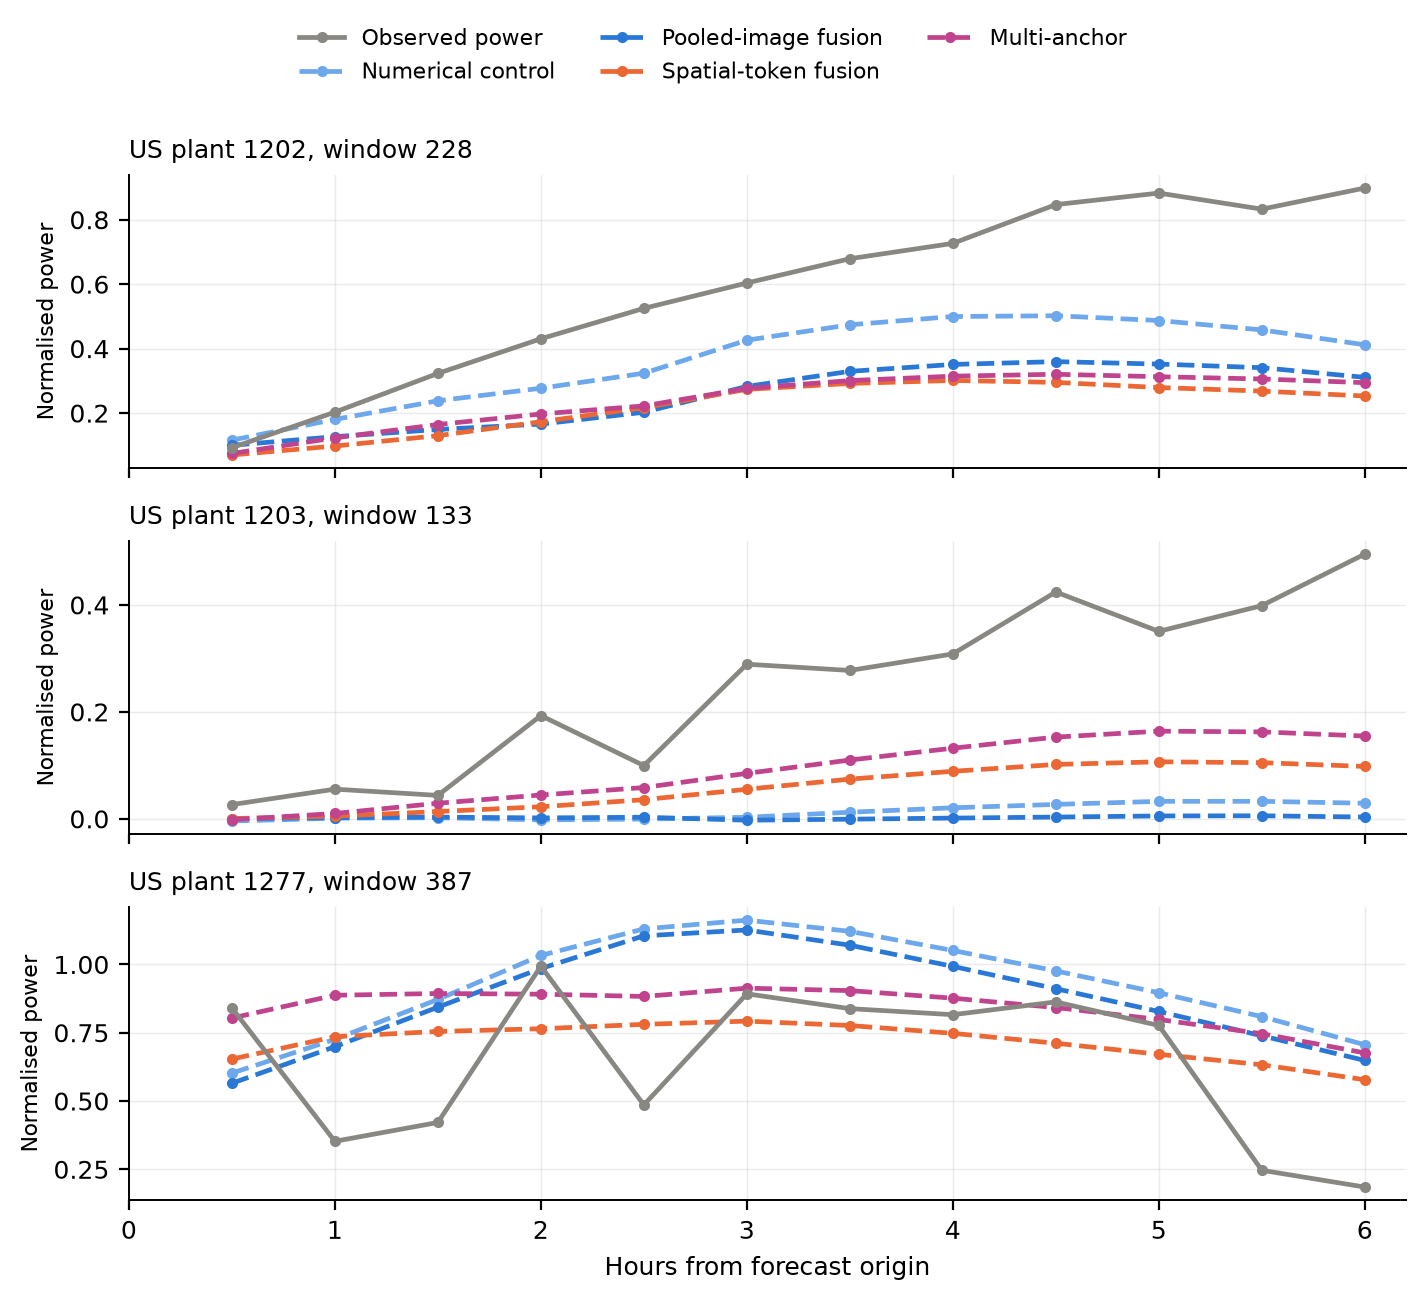
\includegraphics[width=0.92\textwidth]{figures/traces_us.png}
\caption{Six-hour US forecasts from the seed-42 prediction exports across plants 1202, 1203, and 1277. Each panel displays the fully valid daylight window with the largest absolute change between its first and last observed target. Dashed lines denote model forecasts and the solid line represents observed normalized power.}
\label{fig:us-traces}
\end{figure}

At plants 1202 and 1203, all four models underpredict the observed morning climb. The numerical control tracks more of the initial rise at plant 1202, while multi-anchor reaches closest to the peak at plant 1203. At plant 1277, the forecasts stay smooth through midday fluctuations and fail to capture the steep late-afternoon drop. These individual events illustrate how even models with competitive aggregate scores can struggle on localized, high-amplitude transitions when deployed across distinct geographic regions.
